\begin{theorem}
    Пусть $f$ монотонна и $f\geq 0$. Тогда $\bigg|\sum\limits_{k=a}^bf(k)-\int\limits_a^b f(x)dx\bigg|\leq \max \{f(a), f(b)\}$.
\end{theorem}

\begin{proof}
    Пусть $f$ убывает.

    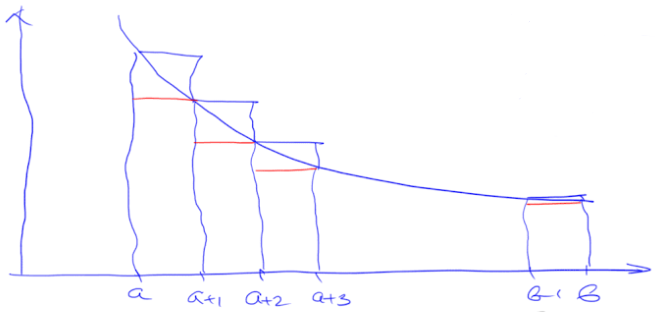
\includegraphics[width=0.5\linewidth]{images/12-04-1.png}

    $\sum\limits_{k=a}^{b-1}f(k)\geq \int\limits_a^b f(x)dx\geq \sum\limits_{k=a+1}^{b}f(k)$

    $\sum\limits_{k=a}^bf(k)-\int\limits_a^b f(x)dx\leq \sum\limits_{k=a}^bf(k) - \sum\limits_{k=a+1}^bf(k)=f(a)$

    $\sum\limits_{k=a}^bf(k)-\int\limits_a^b f(x)dx\geq \sum\limits_{k=a}^bf(k) - \sum\limits_{k=a}^{b-1}f(k)=f(b)$
\end{proof}

\begin{exercise}
    Если $f$ монотонна, то $\bigg|\sum\limits_{k=a}^bf(k)-\int\limits_a^b f(x) dx\bigg|\leq \max \{|f(a)|, |f(b)|\}$.
\end{exercise}

\begin{theorem}
    \textbf{Интегральный признак сходимости ряда (Коши).}

    Пусть $f:[1, +\infty)\rightarrow[0, +\infty)$ монотонно убывает. Тогда $\sum\limits_{k=1}^{+\infty}f(k)$ и $\int\limits_1^{+\infty}f(x) dx$ ведут себя одинаково. 
\end{theorem}

\begin{proof}
    Пусть $S_n:=\sum\limits_{k=1}^n f(k)$ и $F(y):=\int\limits_1^y f(x)dx$.

    Так как все неотрицательно, то:
    
    \begin{enumerate}
        \item $\int\limits_1^\infty f(x)dx$ сходится $\Leftrightarrow F(y)$ ограничена сверху.
        \item $\sum\limits_{k=1}^\infty f(k)$ сходится $\Leftrightarrow S(n)$ ограничена сверху.
    \end{enumerate}

    Поэтому нужно понять, что ограниченность $S_n\Leftrightarrow$ ограниченность $F(n)$.

    $|S_n-F(n)|=\bigg|\sum\limits_{k=1}^n f(k)-\int\limits_1^n f(x)dx\bigg|\leq f(1)$ (по лемме, $f(1)$ – максимум, так как $f$ убывает).

    \begin{enumerate}
        \item[$\Leftarrow$.] Если $S_n\leq M$, то $\int\limits_1^{+\infty}f(x)dx\leq M+f(1)\Rightarrow F(y)\leq M+f(1)$.
        \item[$\Rightarrow$.] Если $F(y)\leq M$, то $S_n\leq M+f(1)$.
    \end{enumerate}
\end{proof}

\begin{example}
    Эта теорема позволяет смотреть на интегралы вместо рядов, чтобы отвечать на вопрос об их сходимости (что иногда проще, чем исследовать на сходимость сам ряд).
    \begin{enumerate}
        \item $\sum\limits_{n=1}^\infty \frac{1}{n^p}$, $p>0$ ведет себя также, как $\int\limits_1^\infty \frac{dx}{x^p}$ – сходится при $p>1$ и расходится при $p\leq 1$.
        \item $\sum\limits_{n=2}^\infty \frac{1}{n\ln n}$ ведет себя также, как $\int\limits_2^\infty \frac{dx}{x\ln x}=\ln \ln x|_2^{+\infty}=+\infty$ расходится.
        \item $\sum\limits_{n=2}^\infty \frac{1}{n^p\ln n}$ ведет себя также, как $\int\limits_2^\infty \frac{dx}{x\ln^p x}=\int\limits_{\ln 2}^\infty\frac{dt}{t^p}$ – сходится при $p>1$ и расходится при $p\leq 1$.
    \end{enumerate}
\end{example}

\begin{corollary}
    Если $0\leq a_n \leq \frac{C}{n^p}$ при $p>1$, то ряд $\sum\limits_{n=1}^{\infty}\frac{C}{n^p}$ сходится.
\end{corollary}
\begin{proof}
    $\sum\limits_{n=1}^{\infty}\frac{1}{n^p}$ – сходится $\Rightarrow$ $\sum\limits_{n=1}^{\infty}\frac{C}{n^p}$ – сходится, а дальше признак сравнения.
\end{proof}

\subsection{Знакопеременные ряды} 
\begin{theorem}
    \textbf{Преобразование Абеля.}
    
    $\sum\limits_{k=1}^na_kb_k=A_nb_n+\sum\limits_{k=1}^{n-1}A_k(b_k-b_{k+1})$, где $A_k=a_1+...+a_k$, $A_0=0$.
\end{theorem}

\begin{proof}
    $\sum\limits_{k=1}^na_kb_k=\sum\limits_{k=1}^n(A_k-A_{k-1})b_k=\sum\limits_{k=1}^nA_kb_k-\sum\limits_{j=2}^nA_{j-1}b_j\overset{j=k+1}{=}\sum\limits_{k=1}^nA_kb_k-\sum\limits_{k=1}^{n-1}A_{k}b_{k+1}=A_nb_n+\sum\limits_{k=1}^{n-1}A_k(b_k-b_{k+1})$
\end{proof}

\begin{remark}
    Получили некоторый дискретный аналог интегрирования по частям (потому что частичная сумма = аналог первообразной, а разность соседних членов ряда = аналог дифференцирования).
\end{remark}

\begin{theorem}
    \textbf{Признак Дирихле.}
    
    $\left \{\begin{array}{l}
        1.\ \sum\limits_{k=1}^na_k\text{ ограничены.} \\
        2.\ b_n\text{ монотонны.} \\
        3.\ \lim b_n=0 
    \end{array}\right.\Rightarrow \sum\limits_{n=1}^\infty a_nb_n$ сходится.
\end{theorem}

\begin{proof}
    Распишем частичную сумму через преобразование Абеля:
    
    $S_n:=\sum\limits_{k=1}^na_k b_k=A_nb_n+\sum\limits_{k=1}^{n-1}A_k(b_k-b_{k+1})\leadsto$ хотим доказать, что $S_n$ имеет предел.
    
    $\lim A_n b_n=0$ – ограниченная $A_n$ на бесконечно малую $b_n$.
    
    $\lim \sum\limits_{k=1}^{n-1}A_k(b_k-b_{k+1})=\sum\limits_{k=1}^\infty A_k(b_k-b_{k+1})$ – если сходится, то сходится к сумме ряда, то есть надо доказать, что ряд сходится. 
    
    Проверим абсолютную сходимость: 
    
    $\sum\limits_{k=1}^\infty|A_k|\cdot|b_k-b_{k+1}|\leq\sum\limits_{k=1}^\infty M\cdot |b_k-b_{k+1}|$ (так как $A_k$ – ограниченны). 
    
    Докажем, что $\sum\limits_{k=1}^n |b_k-b_{k+1}|$ сходится:

    $\sum\limits_{k=1}^n |b_k-b_{k+1}|=\bigg|\sum\limits_{k=1}^n (b_k-b_{k+1})\bigg|$ (разности одного знака, так как $b_n$ монотонны) $=$
    
    $=|(b_1-b_2)+(b_2-b_3)+..+(b_n-{b_{n+1}})|=|b_1-b_{n+1}|\rightarrow b_1\Rightarrow $ частичная сумма сходится $\Rightarrow$ ряд сходится.  
\end{proof}

\begin{theorem}
    \textbf{Признак Абеля}

    $\left \{\begin{array}{l}
        1.\ \sum\limits_{n=1}^\infty a_n\text{ сходится.} \\
        2.\ b_n\text{ монотонны.} \\
        3.\ b_n\text{ ограничены.} 
    \end{array}\right .\Rightarrow \sum\limits_{n=1}^\infty a_nb_n$ сходится.
\end{theorem}

\begin{proof}
    $b_n$ монотонны и ограниченны $\Rightarrow\exists$ конечный $\lim b_n=b$.

    Пусть $\Tilde{b_n}:=b_n-b$, $\Tilde{b_n}$ монотонны и $\lim \Tilde{b_n}=0$.

    Посмотрим на частичные суммы $A_n:=\sum\limits_{k=1}^na_k\rightarrow \sum\limits_{k=1}^\infty a_k\Rightarrow A_n$ ограничена.

    $a_n$ и $\Tilde{b_n}$ удовлетворяют условиям признака Дирихле и тогда $\sum\limits_{n=1}^\infty a_n\Tilde{b_n}$ сходится. 

    $\sum\limits_{n=1}^\infty a_nb_n=\underbrace{\sum\limits_{n=1}^\infty a_n\Tilde{b_n}}_{\text{сх-ся}}+\underbrace{\sum\limits_{n=1}^\infty a_nb}_{=b\sum\limits_{n=1}^\infty a_n\text{ сх-ся по усл.}}\Rightarrow \sum\limits_{n=1}^\infty a_nb_n$ сходится. 
\end{proof}

\begin{exercise}
    $\sum\limits_{n=1}^\infty \frac{\sin n}{n}$ – сходится. Указание – использовать формулу суммы $\sin x$.
\end{exercise}

\begin{example}
    $\sum\limits_{n=1}^\infty \frac{1}{n^3\sin ^2 n}$ неизвестно сходится или нет (конкретно Храброву, и вообще социуму).
\end{example}

\begin{definition}
    Пусть $a_n\geq 0$. Тогда \textit{знакочередующийся ряд} – это ряд $\sum\limits_{n-1}^\infty (-1)^{n-1}a_n=$

    $=a_1-a_2+a_3-...$
\end{definition}

\begin{theorem}
    \textbf{Признак Лейбница.}

    Если $a_n$ монотонно убывают и $\lim a_n=0$, то $\sum\limits_{n-1}^\infty (-1)^{n-1}a_n$ сходится. Более того, $S_{2n}\leq S\leq S_{2n-1}$, где $S$ – сумма ряда, $S_n$ – частичная сумма.
\end{theorem}

\begin{proof}
    $S_{2n+2}=S_{2n}+a_{2n+1}-a_{2_n+2}\geq S_{2n}$

    $S_{2n+1}=S_{2n-1}-a_{2n}+a_{2_n+1}\leq S_{2n-1}$

    $[0, S_1]\supset [S_2, S_3]\supset [S_4, S_5]\supset ...$ и $S_{2n+1}-S_{2n}=a_{2n+1}\rightarrow 0$ – это стягивающиеся отрезки. Тогда есть единственная точка $S$, лежащая во всех отрезках и это предел их концов, то есть предел частичных сумм $\Rightarrow S$ – сумма ряда.
\end{proof}

\begin{example}
    $\sum\limits_{n=1}^{\infty}\frac{(-1)^{n-1}}{n^p}$

    Если $p>0$, то ряд \textit{сходится}, так как $a_n=\frac{1}{n^p}\searrow $.

    Если $p\leq 0$, то ряд \textit{расходится}, так как $a_n\not \rightarrow 0$.
\end{example}

\begin{example}
    \textbf{Ряд Лейбница.}

    $\sum\limits_{k=1}^{\infty}\frac{(-1)^{k-1}}{k}$

    $S_{2n}=1-\frac{1}{2}+\frac{1}{3}-...+\frac{1}{2n-1}-\frac{1}{2n}=1+\frac{1}{2}+\frac{1}{3}+...+\frac{1}{2n-1}+\frac{1}{2n}-2(\frac{1}{2}+\frac{1}{4}+...+\frac{1}{2n})=H_{2n}-H_n=\ln (2n)+\gamma + o(1)-(\ln n + \gamma +o(1))=\ln 2+o(1)\rightarrow \ln 2$.
\end{example}

\begin{example}
    $(1-\frac{1}{2}-\frac{1}{4})+(\frac{1}{3}-\frac{1}{6}-\frac{1}{8})+..+(\frac{1}{2n-1}-\frac{1}{4n-2}-\frac{1}{4n})+...$.

    $\Tilde{S_n}=\sum\limits_{k=1}^n(\underbrace{\frac{1}{2k-1}-\frac{1}{4k-2}}_{=\frac{1}{4k-2}}-\frac{1}{4k})=\frac{1}{2}\sum\limits_{k=1}^n(\frac{1}{2k-1}-\frac{1}{2k})=\frac{1}{2}S_{2n}\rightarrow\frac{\ln 2}{2}$

    Переставили члены ряда и сумма поменялась...
\end{example}

\begin{definition}
    Пусть $\varphi:\N \rightarrow \N$ – биекция, $\sum\limits_{n=1}^\infty a_n$ – ряд. Тогда $\sum\limits_{n=1}^\infty a_{\varphi(n)}$ – \textit{перестановка ряда} $\sum\limits_{n=1}^\infty a_n$.
\end{definition}

\begin{theorem}~
    \begin{enumerate}
        \item Если $a_n\geq 0$, то $\sum\limits_{n=1}^\infty a_{\varphi(n)}=\sum\limits_{n=1}^\infty a_n$ (тут могут быть $+\infty$).
        \item Если ряд абсолютно сходится, то $\sum\limits_{n=1}^\infty a_{\varphi(n)}=\sum\limits_{n=1}^\infty a_n$.
    \end{enumerate}
\end{theorem}
\begin{proof}~
    \begin{enumerate}
        \item Пусть $S_n:=\sum\limits_{k=1}^n a_k$, $\Tilde{S_n}:=\sum\limits_{k=1}^n a_{\varphi(k)}$, $S$  и $\Tilde{S}$ – суммы рядов (существуют, так как слагаемые неотрицательны).

        $\Tilde{S_n}=a_{\varphi(1)}+..+a_{\varphi(n)}\leq S_{\max\{\varphi(1), ..., \varphi(n)\}}\leq S\Rightarrow \underset{\rightarrow\Tilde{S}}{\Tilde{S_n}}\leq S\Rightarrow \Tilde{S}\leq S$. 
        
        Все симметрично, поэтому если мы напишем обратную перестановку, то получим, что $S\leq \Tilde{S}\Rightarrow S= \Tilde{S}$.
        \item Пусть $(a_n)_+=\max\{a_n, 0\}$, $(a_n)_-=\max\{-a_n, 0\}$.

        $0\leq (a_n)_\pm \leq |a_n|$ и $a_n=(a_n)_++(a_n)_-$

        $\sum\limits_{n=1}^\infty |a_n|$ – сходится $\Rightarrow\sum\limits_{n=1}^\infty (a_n)_\pm$ – сходится $\Rightarrow \sum\limits_{n=1}^\infty (a_{\varphi(n)})_\pm$ сходится по тем же суммам (сумма неотрицательных членов).

        $\sum\limits_{n=1}^\infty a_n=\underbrace{\sum\limits_{n=1}^\infty (a_n)_+-\sum\limits_{n=1}^\infty (a_n)_-}_{\text{сх-ся}}=\sum\limits_{n=1}^\infty (a_{\varphi(n)})_+-\sum\limits_{n=1}^\infty (a_{\varphi(n)})_-=\sum\limits_{n=1}^\infty a_{\varphi(n)}$
    \end{enumerate}
\end{proof}

\begin{exercise}
    Доказать 2 для $a_n\in \C$.
\end{exercise}

\begin{definition}
    $\sum a_n$ \textit{сходится условно}, если $\sum a_n$ – сходится, а $\sum |a_n|$ – расходится.
\end{definition}

\begin{remark}
    Если $\sum a_n$ сходится условно, то $\sum\limits_{n=1}^\infty (a_n)_\pm=+\infty.$
\end{remark}

\begin{proof}
    Пусть $\sum\limits_{n=1}^\infty (a_n)_+$ конечна, $(a_n)_-=(a_n)_+-a_n$.

    $\sum (a_n)_-=\underbrace{\sum (a_n)_+-\sum a_n}_{\text{сх-ся}}\Rightarrow \sum (a_n)_-$ сходится.

    $\sum |a_n|=\underbrace{\sum (a_n)_+\sum (a_n)_-}_{\text{сх-ся}}$ сходится. Противоречие.
\end{proof}

\begin{theorem}
    \textbf{Теорема Римана.}

    Пусть $\sum a_n$ сходится условно. Тогда $\forall S\in \overline{\R}$ существует перестановка $\varphi: \N \rightarrow \N$, для которой $\sum a_{\varphi(n)}=S$. Также существует перестановка, для которой ряд не имеет суммы.
\end{theorem}

\begin{proof}
    Берем $(a_n)_+$ и выкидываем все, для которых $a_n\leq 0$, остальное перенумеруем и назовем $b_n$. Берем $(a_n)_-$ и выкидываем все, для которых $a_n>0$, остальное перенумеруем и назовем $c_n$ (разделили все члены ряда на положительные и неположительные).

    $\sum b_n=\sum (a_n)_+=+\infty\quad\sum c_n=\sum (a_n)_-=+\infty$.

    Для каждого $a_n$ есть ровно одна $b_k$ или $c_k$, т.ч. $a_n=b_k$ или $a_n=c_k$ (существует биекция).

    Еще знаем, что $\lim b_n=\lim c_n=0$.

    \begin{enumerate}
        \item $S\in \R$

        Берем $b$-шки до тех пор, пока сумма не перевалит через $S$.

        $b_1+b_2+...+b_{n_1-1}\leq S< b_1+..+b_2+..+b_{n_1}$

        $S_1-b_{n_1} \leq S < S_1$

        Берем $-c$-шки до тех пор, пока сумма не перевалит через $S$.

        $b_1+b_2+...+b_{n_1-1}-c_1-..-c_{m_1-1}< S\leq  b_1+..+b_2+..+b_{n_1}-c_1-..-c_{m_1}$

        $S_2 < S \leq S_2 + c_{m_1}$

        Снова берем $b$-шки до тех пор, пока сумма не перевалит через $S$.

        $b_1+b_2+...+b_{n_1-1}-c_1-..-c_{m_1-1}+b_{n_1+1}+..+b_{n_2-1}\leq S <  b_1+..+b_2+..+b_{n_1}-c_1-..-c_{m_1}+b_{n_1+1}+..+b_{n_2}$

        $S_3-b_{n_2} \leq S < S_3$

        У нас получилась перестановка (на каждом шаге берем какую-то $b$-шку или $c$-шку, пустых шагов не бывает).
        
        Так можно брать, так как ряд $b_n$ и ряд $c_n$ расходящиеся, их сумма может быть сколь угодно большой (иначе сумма была бы конечная с какого-то номера). При этом строгие знаки нужны, чтобы не было пустых шагов.

        Осталось проверить, что сумма полученной перестановки равна $S$. Расставим скобки вокруг блоков с одним знаком и проверим, что такая последовательность частичных сумм стремится к $S$.

        $|S_{2k+1}-S|\leq b_{n_k}\rightarrow 0$

        $|S_{2k}-S|\leq c_{m_k}\rightarrow 0$
        \item $S=+\infty$

        Берем $b$-шки до тех пор, пока сумма не перевалит через $1$ $\leadsto S_1>1$, $\lim S_{2k-1}=+\infty$.

        Берем одну $-c$-шку.
        
        Берем $b$-шки до тех пор, пока сумма не перевалит через $2$ $\leadsto S_3>2$, $\lim S_{2k-1}=+\infty$.

        Берем одну $-c$-шку.

        И так далее. Для $-\infty$ аналогично.

        \item Нет суммы.

        Берем $b$-шки до тех пор, пока сумма не перевалит через $1$ $\leadsto S_1>1$.
        
        Берем $b$-шки до тех пор, пока сумма не перевалит через $-1$ $\leadsto S_2<-1$.

        Берем $b$-шки до тех пор, пока сумма не перевалит через $1$ $\leadsto S_3>1$.

        Берем $b$-шки до тех пор, пока сумма не перевалит через $-1$. И так далее.
    \end{enumerate}
\end{proof}

\begin{theorem}
    \textbf{Теорема Коши о произведении рядов.}

    Если ряды $\sum\limits_{n=1}^\infty a_n=A$ и $\sum\limits_{n=1}^\infty b_n=B$ абсолютно сходящиеся, то ряд, составленный из всевозможных произведений $a_kb_m$, абсолютно сходится и его сумма $AB$.
\end{theorem}

\begin{proof}
    Пусть $A^*=\sum\limits_{n=1}^\infty |a_n|$, $B^*=\sum\limits_{n=1}^\infty |b_n|$.

    Рассмотрим сумму $\sum |a_i b_j|\leq \sum\limits_{i=1}^n|a_i|\cdot \sum\limits_{j=1}^m|b_j|\leq A^*\cdot B^*$, где $n$ – наибольший из индексов $i$, встречающийся слева, $m$ – наибольший из индексов $j$, встречающийся слева

    $\Rightarrow \sum\limits_{i, j=1}^\infty |a_i b_j|$ абсолютно сходящийся $\Rightarrow$ сумма ряда $\sum\limits_{i, j=1}^\infty a_i b_j$ не зависит от порядка суммирования.

    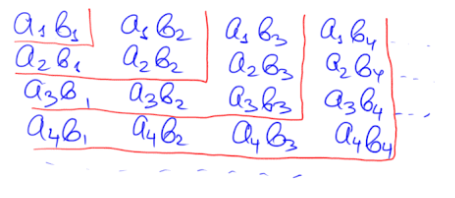
\includegraphics[width=0.4\linewidth]{images/12-04-2.png}
    
    $S_{n^2}=\sum\limits_{i=1}^n\sum\limits_{j=1}^n a_ib_j=\underset{\rightarrow A}{\sum\limits_{i=1}^na_i}\cdot \underset{\rightarrow B}{\sum\limits_{j=1}^n b_j}\rightarrow AB$

    $\lim S_{n^2}=AB\Rightarrow S= AB$.
\end{proof}

\begin{definition}
    \textit{Произведение рядов} $\sum\limits_{n=1}^\infty a_n$ и $\sum\limits_{n=1}^\infty b_n$ – ряд $\sum\limits_{n=1}^\infty c_n$, где $c_n=a_1b_n+a_2b_{n-1}+...+a_nb_1$.

    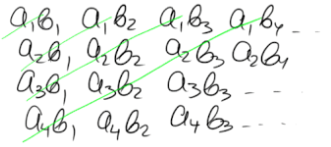
\includegraphics[width=0.35\linewidth]{images/12-04-3.png}
\end{definition}

\begin{remark}
    Из теоремы Коши следует, что если $\sum\limits_{n=1}^\infty a_n$ и $\sum\limits_{n=1}^\infty b_n$ абсолютно сходится, то $\sum\limits_{n=1}^\infty c_n$ абсолютно сходится и $\sum\limits_{n=1}^\infty a_n\cdot \sum\limits_{n=1}^\infty b_n$=$\sum\limits_{n=1}^\infty c_n$.
\end{remark}

\begin{theorem}
    \textbf{Теорема Мертенса.}

    Если $\sum\limits_{n=1}^\infty a_n=A$ и $\sum\limits_{n=1}^\infty b_n=B$ и один из рядов абсолютно сходящийся, то $\sum\limits_{n=1}^\infty c_n$ сходится и $\sum\limits_{n=1}^\infty c_n=AB$.
\end{theorem}

\begin{proof}
    Не будет.
\end{proof}

\begin{remark}~
    \begin{enumerate}
        \item Здесь важен порядок суммирования, так как нет абсолютной сходимости.
        \item Обычно сходимости не хватает.
    \end{enumerate}
\end{remark}

\begin{example}
    $a_n=b_n=\frac{(-1)^{n-1}}{\sqrt{n}}$, $\sum\limits_{n=1}^\infty a_n$ и $\sum\limits_{n=1}^\infty b_n$ сходятся, но не абсолютно.

    $c_n=(-1)^{n-1}(\frac{1}{\sqrt{1}}\cdot \frac{1}{\sqrt{n}}+\frac{1}{\sqrt{2}}\cdot \frac{1}{\sqrt{n-1}}+...+\frac{1}{\sqrt{n}}\cdot \frac{1}{\sqrt{1}})$

    Каждое слагаемое не меньше $\frac{1}{n}$: $\frac{1}{\sqrt{k}}\cdot \frac{1}{\sqrt{n-k}}\geq \frac{1}{n}$

    $n^2\geq k(n-k)$

    Тогда $|c_n|\geq n\cdot \frac{1}{n}=1$ и ряд расходится, так как $c_n\not \rightarrow 0$.
\end{example}

\begin{theorem}
    \textbf{Теорема Абеля.}

    Если $\sum\limits_{n=1}^\infty a_n=A$, $\sum\limits_{n=1}^\infty b_n=B$ и $\sum\limits_{n=1}^\infty c_n=C$, где $c_n=a_1b_n+..+a_nb_1$, то $AB=C$.
\end{theorem}

\begin{lemma}
     Пусть $\lim x_n=x$, $\lim y_n=y$ – конечные пределы. Тогда $\frac{x_1y_n+...+x_ny_1}{n}\rightarrow xy$.
\end{lemma}

\begin{proof}~
    \begin{enumerate}
        \item Пусть $y=0$. Надо доказать, что $x_1y_n+...+x_ny_1=o(n)$.

        $|x_n|\leq M$, $|y_n|\leq M$, $\lim y_n=0\Rightarrow \exists N\ \forall n\geq N\ |y_n|<\varepsilon$.

        $|x_1y_n+...+x_ny_1|\leq \underset{<\varepsilon M}{|x_1y_n|}+\underset{<\varepsilon M}{|x_2y_{n-1}|}...+\underset{\leq M^2}{|x_{n-N+1}y_N|}+...+\underset{\leq M^2}{|x_ny_1|}< (n-N+1)\varepsilon M + (N-1)M^2$

        $\frac{x_1y_n+...+x_ny_1}{n}< \underset{<1}{(1-\frac{N-1}{n})}\varepsilon M + \underset{<\varepsilon \text{ при больших }n}{\frac{N-1}{n}}M^2< \varepsilon M + \varepsilon$

        \item Пусть $y_n=y$.

        $\frac{x_1y_n+...+x_ny_1}{n}=y\cdot \frac{x_1+...+x_n}{n}\rightarrow xy$ (по следствию из теоремы Штольца).

        \item Общий случай $\Tilde{y_n}=y_n-y\rightarrow 0$
    
        $\frac{x_1\Tilde{y_n}+...+x_n\Tilde{y_1}}{n}\rightarrow 0$, $\frac{x_1y+...+x_ny}{n}\rightarrow xy$ и сложим.
    \end{enumerate}
\end{proof}

\begin{proof}
    Пусть $A_n:=\sum\limits_{n=1}^n a_k$, $B_n:=\sum\limits_{n=1}^n b_k$ и $C_n:=\sum\limits_{n=1}^n c_k$.

    По лемме знаем, что $\frac{A_1B_n+...+A_nB_1}{n}\rightarrow AB$.

    $\frac{A_1B_n+...+A_nB_1}{n}=\frac{1}{n}(na_1b_2+(n-1)(a_1b_2+a_2b_1)+(n-2)(a_1b_3+a_2b_2+a_3b_1)+...+(a_1b_n+...+a_nb_1))=\frac{nc_1+(n-1)c_2+...+c_n}{n}=\frac{C_1+...+C_n}{n}\rightarrow C$
\end{proof}

\subsection{Бесконечные произведения}

\begin{definition}
    $\prod\limits_{n=1}^\infty x_n$ – \textit{бесконечное произведение},  $P_n:=x_1x_2...x_n$ – \textit{частичное произведение}.

    Если существует $\lim P_n$, то его называют \textit{значением бесконечного произведения}.

    Если он конечен и отличен от $0$, то бесконечное проивзедение \textit{сходится}.
\end{definition}

\begin{example}~
    \begin{enumerate}
        \item $\prod\limits_{n=2}^\infty(1-\frac{1}{n^2})=\frac{1}{2}$

        $P_n=(1-\frac{1}{2^2})(1-\frac{1}{3^2})...(1-\frac{1}{n^2})=\frac{(2^2-1)(3^2-1)...(n^2-1)}{2^2\cdot 3^2\cdot...\cdot n^2}=\frac{1\cdot 3\cdot 2\cdot 4...\cdot (n-1)(n+1)}{2^2\cdot 3^2\cdot...\cdot n^2}=\frac{n+1}{2n}\rightarrow \frac{1}{2}$

        \item $\prod\limits_{n=1}^\infty(1-\frac{1}{4n^2})=\frac{2}{\pi}$

        $P_n=(1-\frac{1}{2^2})(1-\frac{1}{4^2})...(1-\frac{1}{(2n)^2})=\frac{1\cdot 3\cdot 3\cdot 5\cdot 5\cdot 7\cdot ...\cdot (2n-1)(2n+1)}{2^2\cdot 4^2\cdot...\cdot (2n)^2}=\frac{(2n+1)((2n-1)!!)^2}{((2n)!!)^2}\rightarrow \frac{2}{\pi}$
    \end{enumerate}
\end{example}

\begin{exercise}~
    \begin{enumerate}
        \item $\prod\limits_{n=1}^\infty(1-\frac{1}{(2n-1)^2})=\frac{\pi}{4}$.   
        \item $\prod\limits_{n=1}^\infty(1+x^{2^{n-1}})=\frac{1}{1-x}$ при $|x|<1$.   
    \end{enumerate}
\end{exercise}

\begin{statement} \textbf{Свойства бесконечного произведения:}
    \begin{enumerate}
        \item Конечное число ненулевых начальных множителей не влияет на сходимость.

        \textit{Комментарий:} добавляется константа, на которую нужно умножать, на существование предела не влияет.
        \item Если $\prod \limits_{n=1}^\infty x_n$ сходится, то $\lim x_n =1$.

        \begin{proof}
            $x_n=\frac{P_n}{P_{n-1}}\rightarrow \frac{P}{P}=1$, если $P=\prod \limits_{n=1}^\infty x_n$. пользуемся тем, что $P\neq 0$ и $P\neq \pm \infty$.
        \end{proof}
        \item У сходящегося произведения все сомножители, начиная с некоторого номера, положительны.

        \textit{Комментарий:} стремятся к 1 $\Rightarrow$ можно рассматривать только такие произведения.

        \item Если $x_n>0$, то для сходимости $\prod \limits_{n=1}^\infty x_n$ необходимо и достаточно сходимости ряда $\sum \limits_{n=1}^\infty\ln x_n$. Если $L$ – сумма ряда, то $P=e^L$.

        \begin{proof}
            $S_n=\sum \limits_{n=1}^\infty\ln x_n\Leftrightarrow P=\prod \limits_{n=1}^\infty x_n=e^{S_n}$.
        \end{proof}
    \end{enumerate}
\end{statement}

